\documentclass[tikz,border=5pt]{standalone}
\usepackage{pgfplots}
\usepgfplotslibrary{groupplots,fillbetween}
\pgfplotsset{compat=1.18}

\definecolor{velocityblue}{RGB}{30,105,175}
\definecolor{pressureorange}{RGB}{210,95,35}
\definecolor{stenosisgray}{RGB}{225,225,225}

\begin{document}
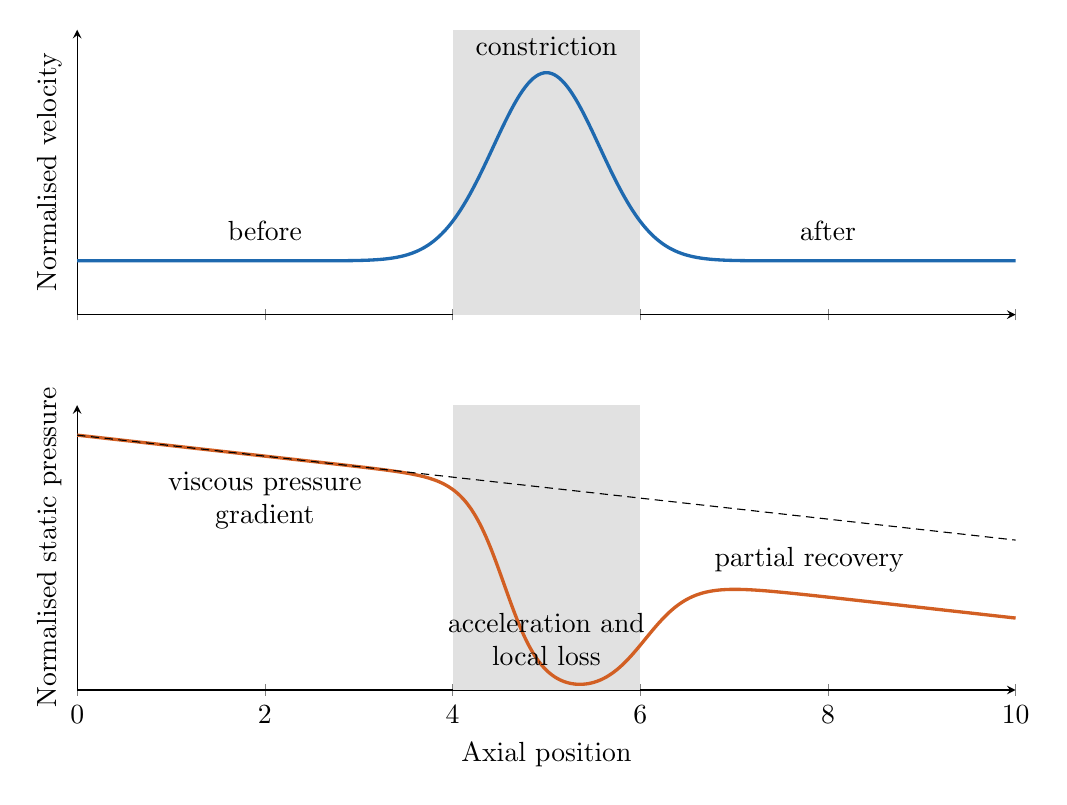
\begin{tikzpicture}
\begin{groupplot}[
  group style={group size=1 by 2, vertical sep=1.15cm},
  width=13.5cm,
  height=5.2cm,
  xmin=0, xmax=10,
  xtick={0,2,4,6,8,10},
  ytick=\empty,
  axis lines=left,
  enlargelimits=false,
  clip=false,
  every axis plot/.append style={very thick, smooth, samples=180},
]

\nextgroupplot[
  ylabel={Normalised velocity},
  xticklabels=\empty,
  ymin=0.5, ymax=3.15,
]
\path[name path=top] (axis cs:4,3.15) -- (axis cs:6,3.15);
\path[name path=bottom] (axis cs:4,0.5) -- (axis cs:6,0.5);
\addplot[stenosisgray] fill between[of=top and bottom];
\addplot[velocityblue,domain=0:10]
  {1 + 1.75*exp(-((x-5)/0.8)^2)};
\node[anchor=south] at (axis cs:2,1.1) {before};
\node[anchor=south] at (axis cs:5,2.82) {constriction};
\node[anchor=south] at (axis cs:8,1.1) {after};

\nextgroupplot[
  xlabel={Axial position},
  ylabel={Normalised static pressure},
  ymin=0.15, ymax=1.1,
]
\path[name path=top2] (axis cs:4,1.1) -- (axis cs:6,1.1);
\path[name path=bottom2] (axis cs:4,0.15) -- (axis cs:6,0.15);
\addplot[stenosisgray] fill between[of=top2 and bottom2];
\addplot[pressureorange,domain=0:10]
  {1 - 0.035*x - 0.68/(1+exp(-5*(x-4.55)))
     + 0.42/(1+exp(-4*(x-6.05)))};
\draw[densely dashed] (axis cs:0,1) -- (axis cs:10,0.65);
\node[anchor=north,align=center] at (axis cs:2,0.91)
  {viscous pressure\\gradient};
\node[anchor=north,align=center] at (axis cs:5,0.44)
  {acceleration and\\local loss};
\node[anchor=south,align=center] at (axis cs:7.8,0.51)
  {partial recovery};

\end{groupplot}
\end{tikzpicture}
\end{document}
